\chapter{Keanekaragaman Organisme Bersel Tunggal}\label{ch:b2:unicellular-diversity}

Setetes air kolam di bawah mikroskop memuat sebuah sel hijau yang
mendayung dengan dua flagelum, seekor siliata berbentuk selop yang
menyapu bakteri ke dalam kerongkongannya, sebuah diatom sebening kaca
yang meluncur di atas kaca objek, dan --- terlalu kecil untuk terlihat
jelas --- seribu bakteri. Masing-masing adalah satu sel dan sekaligus
satu organisme utuh: ia makan, bergerak, mengindera, tumbuh, berbiak,
lalu mati sebagai sel tunggal. Sebagian besar dunia kehidupan memang
selalu seperti itu. Bab ini memandang \omterm{def:b2:unicellular-diversity:unicellular}{organisme bersel tunggal} sebagai
sebuah masalah rancangan --- apa yang dapat dan tidak dapat dikerjakan
satu sel --- lalu menelusuri jawaban yang ditemukan \omterm{def:b2:unicellular-diversity:prokaryote}{prokariot} dan
eukariot, sampai ke titik ketika sel mulai tinggal bersama.

\section{Satu sel, seluruh fungsinya}

\begin{definition}[Bersel tunggal, berkoloni, bersel banyak]\label{def:b2:unicellular-diversity:unicellular}
Sebuah organisme disebut \emph{bersel
tunggal}\index{organisme bersel tunggal} apabila satu sel menjalankan
setiap fungsi kehidupan ---
nutrisi, pertukaran, gerak, perkembangbiakan --- dan hidup sendiri. Ia
\emph{berkoloni}\index{organisme berkoloni} apabila sel-sel sejenis
tetap melekat sesudah membelah tetapi masing-masing masih sanggup hidup
sendiri bila dipisahkan. Ia \emph{bersel
banyak}\index{organisme bersel banyak} apabila sel-selnya terdiri atas
beberapa tipe, saling bergantung, dan hanya sedikit di antaranya (garis
nutfah) yang meninggalkan keturunan. Organisme bersel tunggal mencakup
seluruh arkea, hampir seluruh bakteri, dan sebagian besar garis
keturunan eukariot; sebutan tak resmi \emph{\omterm{def:b2:unicellular-diversity:protist}{protista}} mencakup eukariot
bersel tunggal, yang bukan satu kelompok melainkan banyak kelompok.
\end{definition}

\begin{example}[Enam penghuni satu tetes]\label{ex:b2:unicellular-diversity:drop}
\emph{Escherichia coli}, sebuah batang sepanjang \qty{2}{\micro m},
berenang dengan seberkas flagelum dan membelah tiap dua puluh menit
bila cukup makan. \emph{Chlamydomonas}, sejenis alga hijau berukuran
\qty{10}{\micro m}, mendayung dengan dua flagelum menuju cahaya yang
dideteksinya lewat bintik mata. \emph{Paramecium}, siliata sepanjang
\qty{200}{\micro m}, berselimut ribuan silia, makan lewat kerongkongan
dan menimba air keluar dengan dua \omterm{prop:b2:unicellular-diversity:osmoregulation}{vakuola kontraktil}. Sebuah diatom
tinggal di dalam cangkang silika berkeping dua yang berhias liang.
\emph{Amoeba} mengalir dengan menjulurkan pseudopodium lalu menelan apa
pun yang ditemuinya. Sebuah sel ragi menumbuhkan tunas anak di
sisinya. Enam jawaban, sangat berbeda ukuran dan permesinannya, atas
satu masalah yang sama.
\end{example}

\begin{omfigure}
\begin{tikzpicture}[x=1.9cm]
  % log scale from 0.1 um to 100 mm : position = log10(size in um) + 1
  \draw[thick] (0,0) -- (6,0);
  \foreach \p/\l in {0/{\qty{0.1}{\micro m}},1/{\qty{1}{\micro m}},2/{\qty{10}{\micro m}},3/{\qty{100}{\micro m}},4/{\qty{1}{mm}},5/{\qty{10}{mm}},6/{\qty{100}{mm}}}
    \draw (\p,0.12) -- (\p,-0.12) node[below, font=\scriptsize] {\l};
  \foreach \p/\c/\l in {0.5/omDef/mikoplasma, 1.3/omDef/{\emph{E.~coli}}, 1.7/omDef/ragi, 2.0/omProp/{\emph{Chlamydomonas}}, 2.7/omProp/diatom, 3.3/omProp/{\emph{Paramecium}}, 3.65/omProp/{\emph{Amoeba proteus}}, 3.9/omThm/{\emph{Thiomargarita} (sebuah bakteri)}, 5.7/omProp/{\emph{Acetabularia}}}
    { \fill[\c] (\p,0) circle (0.05); \node[rotate=60, anchor=west, font=\scriptsize, \c, inner sep=1pt] at (\p,0.12) {\l}; }
  \node[font=\scriptsize, anchor=north] at (3,-0.55) {ukuran sel (skala logaritmik)};
\end{tikzpicture}

{\small Ukuran \omterm{def:b2:unicellular-diversity:unicellular}{organisme bersel tunggal} terentang lima orde besar.
\omterm{def:b2:unicellular-diversity:prokaryote}{Prokariot} (biru) mengerumun di sekitar satu mikrometer; sel eukariot
(jingga) sepuluh sampai seratus kali lebih besar; sel tunggal yang
terbesar --- sebuah bakteri belerang raksasa, alga \emph{Acetabularia}
--- adalah kekecualian yang dijelaskan teksnya.}
\end{omfigure}

\begin{proposition}[Permukaan, volume, dan batas ukuran]\label{prop:b2:unicellular-diversity:surface}
\index{rasio permukaan terhadap volume}
Sebuah sel bertukar dengan sekelilingnya lewat permukaannya dan
mengonsumsi sebanding dengan volumenya. Untuk sebuah bola berjari-jari
$r$, \emph{\omterm{prop:b2:unicellular-diversity:surface}{rasio permukaan terhadap volume}}nya adalah
\[
\frac{S}{V} = \frac{4\pi r^2}{\tfrac{4}{3}\pi r^3} = \frac{3}{r},
\]
sehingga melipatduakan jari-jarinya memerohkan separuh permukaan yang
tersedia tiap satuan sitoplasma. Maka sel yang mengandalkan difusi
menyeberangi membrannya untuk memberi makan bagian dalamnya tidak dapat
tumbuh tanpa batas: pada suatu jari-jari, pasokan lewat permukaannya
tidak lagi mengimbangi permintaan volumenya. Hukum yang sama
menjelaskan mengapa sel kecil paling giat bermetabolisme tiap gramnya,
dan mengapa sel besar berbentuk pipih, memanjang, bervakuola, atau
penuh membran dalam.
\end{proposition}

\begin{theorem}[Waktu difusi menempuh suatu jarak]\label{thm:b2:unicellular-diversity:diffusion}
\index{waktu difusi}
Sebuah molekul dengan koefisien difusi $D$ mengembara dalam langkah
acak; sesudah waktu $t$ purata kuadrat simpangannya pada satu sumbu
adalah $\langle x^2\rangle = 2Dt$. Maka waktu yang dibutuhkan untuk
menempuh jarak $x$ dengan difusi semata adalah
\[
t \approx \frac{x^2}{2D},
\]
yang tumbuh dengan \emph{kuadrat} jaraknya. Dengan
$D \approx \qty{1e-9}{m^2/s}$ bagi molekul kecil di dalam air,
menyeberangi sebuah bakteri (\qty{1}{\micro m}) memakan setengah
milidetik; menyeberangi sel \qty{1}{mm} memakan delapan menit, dan satu
meter, enam belas tahun.
\end{theorem}
\begin{proof}
Misalkan molekulnya melangkah sepanjang $\ell$ secara acak ke kiri atau
ke kanan tiap $\tau$ sekon. Sesudah $n$ langkah simpangannya adalah
$x = \sum_i \varepsilon_i \ell$ dengan $\varepsilon_i = \pm 1$ yang
saling bebas, sehingga $\langle x\rangle = 0$ dan $\langle x^2\rangle =
\sum_i \langle\varepsilon_i^2\rangle \ell^2 = n\ell^2$ (suku silangnya
rata-rata nol). Dengan $n = t/\tau$ ini menjadi $\langle x^2\rangle
= (\ell^2/\tau)\,t$, dan dengan menuliskan $D = \ell^2/2\tau$ diperoleh
$\langle x^2\rangle = 2Dt$. Menetapkan $\langle x^2\rangle = x^2$
memberikan waktunya.
\end{proof}

\begin{theorem}[Pasokan difusif ke sel berbentuk bola]\label{thm:b2:unicellular-diversity:supply}
\index{penyerapan terbatas difusi}
Sebuah sel bola berjari-jari $r_0$ yang menyerap setiap molekul zat
terlarut yang mencapai permukaannya, di dalam medium yang
kepekatannya jauh di kejauhan adalah $c_\infty$, menerima fluks (molekul
tiap sekon) pada keadaan tunak sebesar
\[
J = 4\pi D r_0\, c_\infty .
\]
Pasokannya hanya tumbuh dengan $r_0$, sedangkan permintaannya tumbuh
dengan $r_0^3$: melewati jari-jari tertentu, sel yang disuapi difusi
akan kelaparan.
\end{theorem}
\begin{proof}
Pada keadaan tunak, cacah molekul yang menyeberangi tiap bola
berjari-jari $r > r_0$ tiap sekon adalah sama, $J = 4\pi r^2 D\,
(\mathrm{d}c/\mathrm{d}r)$ (hukum Fick, dengan fluksnya terarah ke
dalam). Jadi $r^2\,\mathrm{d}c/\mathrm{d}r = J/4\pi D$ tetap;
mengintegralkan dari $r_0$, tempat $c = 0$, sampai tak hingga, tempat
$c = c_\infty$: $c_\infty = (J/4\pi D)\int_{r_0}^{\infty} r^{-2}\,\mathrm{d}r =
J/(4\pi D r_0)$, sehingga $J = 4\pi D r_0 c_\infty$.
\end{proof}

\begin{example}[Seberapa besar sel yang disuapi difusi?]\label{ex:b2:unicellular-diversity:howbig}
Sebuah sel aerob mengonsumsi oksigen kira-kira $q = \qty{0.02}{mol/m^3/s}$
sitoplasma (laju yang cukup deras). Permintaannya adalah $q \cdot \tfrac{4}{3}\pi
r_0^3$; pasokan dari air jenuh udara ($c_\infty =
\qty{0.25}{mol/m^3}$, $D = \qty{2e-9}{m^2/s}$) adalah $4\pi D r_0
c_\infty$. Menyamakan keduanya, $r_0^2 = 3Dc_\infty/q = 3\times 2\times 10^{-9}
\times 0.25/0.02 = \qty{7.5e-8}{m^2}$, sehingga $r_0 \approx
\qty{270}{\micro m}$. Sel nyata yang giat tinggal jauh di bawah angka ini
karena oksigennya masih harus berdifusi \emph{di dalam} sel itu sendiri;
bakteri belerang \qty{750}{\micro m} \emph{Thiomargarita} mengelak dari
batas ini dengan menjadi hampir seluruhnya vakuola, sitoplasmanya
sekadar selaput tipis setebal beberapa mikrometer.
\end{example}

\begin{omfigure}
\begin{tikzpicture}
\begin{axis}[
  width=0.8\linewidth, height=6.2cm,
  axis x line=bottom, axis y line=left,
  xmode=log, ymode=log,
  xmin=0.3, xmax=1000, ymin=1e-6, ymax=1e4,
  xlabel={jari-jari sel (\unit{\micro m})}, ylabel={molekul tiap sekon (relatif)},
  xlabel style={font=\small, at={(axis description cs:0.5,-0.1)}, anchor=north},
  ylabel style={font=\small},
  tick label style={font=\small},
  legend style={font=\small, at={(0.03,0.97)}, anchor=north west, draw=none},
  clip=false,
]
\addplot[very thick, omDef, domain=0.3:1000, samples=40] {x/10};
\addlegendentry{pasokan oleh difusi, $\propto r$}
\addplot[very thick, omThm, domain=0.3:1000, samples=40] {(x/10)^3/1000*1.0};
\addlegendentry{permintaan sitoplasma, $\propto r^3$}
\draw[dashed, gray] (axis cs:270,1e-6) -- (axis cs:270,27);
\node[font=\scriptsize, anchor=west] at (axis cs:300,3e-4) {jari-jari kelaparan};
\end{axis}
\end{tikzpicture}

{\small Pasokan lewat permukaan tumbuh dengan $r$, permintaan dengan
$r^3$ (sumbu logaritmik). Di tempat kedua garisnya berpotongan, sel yang
hanya disuapi difusi tidak lagi sanggup memasok bagian dalamnya;
perpotongannya terletak di sekitar beberapa ratus mikrometer bagi sel
aerob yang giat.}
\end{omfigure}

\section{Keanekaragaman prokariot}

\begin{definition}[Sel prokariot]\label{def:b2:unicellular-diversity:prokaryote}
Sebuah \emph{prokariot}\index{prokariot} (bakteri dan arkea, dua domain
yang satu sama lain sejauh jarak masing-masing dari kita) adalah sel
tanpa nukleus maupun organel bermembran: satu kromosom melingkar di
dalam sebuah \emph{nukleoid}\index{nukleoid}, kerap disertai lingkaran
kecil tambahan yang disebut \emph{plasmid}\index{plasmid}, ribosom yang
bebas di dalam sitoplasma berukuran \qtyrange{0.5}{2}{\micro m}, sebuah
membran plasma yang mengusung rantai respirasi atau fotosintesis, dan
sebuah \emph{dinding sel}\index{dinding sel!bakteri} kaku yang menahan
turgor sitoplasma beberapa bar di atas sekelilingnya. Bentuknya sedikit
dan bernama: \emph{kokus} (bola), \emph{basil} (batang),
\emph{spirilum} dan \emph{spiroket} (heliks), \emph{vibrio} (koma);
selnya dapat tetap berpasangan, berantai, bertetrad, atau bergerombol
sesudah membelah.
\end{definition}

\begin{proposition}[Dua selubung: Gram positif dan Gram negatif]\label{prop:b2:unicellular-diversity:gram}
\index{pewarnaan Gram}\index{peptidoglikan}
Dinding bakteri tersusun atas \emph{peptidoglikan}, yaitu rantai dua
gula berselang-seling yang bertaut silang lewat peptida pendek menjadi
satu molekul raksasa yang mengelilingi selnya. Bakteri \emph{Gram
positif} memiliki lapisan tebal (\qtyrange{20}{80}{nm}) di luar satu
membran dan menahan zat warna kristal ungu pada prosedur Gram; bakteri
\emph{Gram negatif} memiliki lapisan tipis (beberapa nanometer) yang
terapit antara membran plasma dan sebuah \emph{membran luar} yang
lembar luarnya terbuat dari lipopolisakarida, dan zat warnanya luruh.
Membran luar itu, yang tertembus porin, adalah penghalang kedua: ia
menahan banyak antibiotik dan deterjen, dan itulah sebabnya jangkitan
Gram negatif lebih sukar diobati. Arkea tidak memiliki peptidoglikan
maupun lipid bertaut ester seperti sel lainnya: membrannya tersusun
atas rantai isoprenoid bertaut eter, kadang merentang seluruh lapis
ganda sebagai satu lapis tunggal, yang membuatnya tetap mantap di dalam
asam mendidih.
\end{proposition}

\begin{omfigure}
\begin{tikzpicture}[scale=0.9, every node/.style={font=\scriptsize}]
  % Gram-positive
  \begin{scope}
    \fill[omDef!15] (0,0) rectangle (4,1.6);
    \node at (2,0.4) {sitoplasma};
    \fill[omDef!60] (0,1.6) rectangle (4,1.85);
    \node[right] at (4.05,1.72) {membran plasma};
    \fill[omProp!50] (0,1.85) rectangle (4,3.0);
    \foreach \y in {2.0,2.25,...,2.85} \draw[omProp!90!black] (0.1,\y) -- (3.9,\y);
    \node[right, align=left] at (4.05,2.45) {peptidoglikan tebal\\(\qtyrange{20}{80}{nm})};
    \node[above, font=\small\bfseries] at (2,3.05) {Gram positif};
  \end{scope}
  % Gram-negative
  \begin{scope}[xshift=7.6cm]
    \fill[omDef!15] (0,0) rectangle (4,1.6);
    \node at (2,0.4) {sitoplasma};
    \fill[omDef!60] (0,1.6) rectangle (4,1.85);
    \node[right] at (4.05,1.72) {membran plasma};
    \fill[omProp!50] (0,2.05) rectangle (4,2.25);
    \draw[omProp!90!black] (0.1,2.15) -- (3.9,2.15);
    \node[right] at (4.05,2.15) {peptidoglikan tipis};
    \node at (2,1.95) {periplasma};
    \fill[omThm!50] (0,2.55) rectangle (4,2.85);
    \foreach \x in {0.6,2.0,3.4} \fill[white] (\x-0.12,2.55) rectangle (\x+0.12,2.85);
    \node[right] at (4.05,2.7) {membran luar berporin};
    \foreach \x in {0.2,0.5,...,3.9} \draw[omThm!80!black, thick] (\x,2.85) -- (\x,3.1);
    \node[right] at (4.05,3.15) {lipopolisakarida};
    \node[above, font=\small\bfseries] at (2,3.3) {Gram negatif};
  \end{scope}
\end{tikzpicture}

{\small Kedua selubung bakteri dalam potongan melintang. Kiri: satu
membran di bawah mantel peptidoglikan yang tebal. Kanan: lapisan
peptidoglikan tipis di dalam periplasma antara dua membran, membran
luarnya bertabur porin dan berselaput lipopolisakarida.}
\end{omfigure}

\begin{proposition}[Flagelum bakteri dan kemotaksis]\label{prop:b2:unicellular-diversity:flagellum}
\index{flagelum!bakteri}\index{kemotaksis}
\emph{Flagelum} bakteri adalah filamen heliks kaku dari protein
flagelin, setebal \qty{20}{nm} dan sepanjang beberapa kali panjang
tubuhnya, yang diputar oleh motor berputar yang terpasang pada
selubungnya. Motornya digerakkan bukan oleh ATP melainkan oleh proton
yang mengalir menuruni landaian elektrokimia melintasi membrannya,
dengan sekitar \num{1000} proton tiap putaran dan sampai \num{300}
putaran tiap sekon. Pada \emph{E.~coli} beberapa flagelumnya berhimpun
menjadi satu berkas ketika semuanya berputar berlawanan arah jarum jam
dan mendorong selnya dalam sebuah \emph{lari} lurus; ketika satu atau
lebih membalik arah, berkasnya berhamburan dan selnya
\emph{terjungkal} ke arah acak yang baru. \emph{Kemotaksis} adalah
kecondongan jalan acak ini: selnya mengukur apakah kepekatan zat
penarik telah naik selama sekon terakhir dan, kalau ya, menekan
jungkalannya. Ia mengemudi dengan membandingkan saat ini dengan masa
lalu yang dekat --- sepanjang lintasannya --- karena sepanjang
\qty{1}{\micro m} tubuhnya sendiri tidak ada landaian yang terukur.
\end{proposition}
\begin{proof}[Bukti eksperimental]
Berg dan Brown (1972) mengikuti sel \emph{E.~coli} tunggal dalam tiga
dimensi dengan mikroskop penjejak: lari sepanjang kira-kira satu sekon
pada \qty{20}{\micro m/s}, jungkalan sepersepuluh sekon, dan di dalam
landaian serina lari yang menaiki landaiannya lebih panjang sedangkan
lari yang menuruninya tidak diperpendek. Menambatkan sebuah sel pada
kaca objek lewat satu flagelum membuat seluruh tubuhnya berputar, yang
membuktikan motornya memang berputar; sel yang motornya diputus dari
sintesis ATP tetap berenang selama landaian proton dapat dipaksakan,
yang menetapkan bahan bakarnya.
\end{proof}

\begin{omfigure}
\begin{tikzpicture}[every node/.style={font=\scriptsize}]
  % run and tumble path without gradient
  \begin{scope}
    \draw[very thick, omDef] (0,0) -- (1.2,0.5) -- (0.7,1.4) -- (1.9,1.8) -- (2.6,0.9) -- (3.4,1.5) -- (3.0,2.5);
    \foreach \p in {(1.2,0.5),(0.7,1.4),(1.9,1.8),(2.6,0.9),(3.4,1.5)} \fill[omThm] \p circle (0.06);
    \node[align=center] at (1.8,-0.5) {tanpa landaian:\\lari sama panjang, belokan acak};
  \end{scope}
  \begin{scope}[xshift=6cm]
    \shade[left color=white, right color=omExo!50] (-0.3,-0.2) rectangle (5.2,3.0);
    \draw[very thick, omDef] (0,0.3) -- (0.9,0.8) -- (0.6,1.3) -- (2.4,1.5) -- (2.2,2.2) -- (4.6,2.4);
    \foreach \p in {(0.9,0.8),(0.6,1.3),(2.4,1.5),(2.2,2.2)} \fill[omThm] \p circle (0.06);
    \node[align=center] at (2.4,-0.5) {zat penarik meningkat ke kanan:\\lari yang menaiki landaian lebih lama};
    \node[anchor=south east] at (5.1,2.6) {zat penarik lebih banyak};
  \end{scope}
\end{tikzpicture}

{\small Lari dan jungkal. Kiri: tanpa landaian, selnya menjalani jalan
acak, tiap larinya (biru) diakhiri sebuah jungkalan (titik merah).
Kanan: ketika zat penarik meningkat sepanjang sebuah lari, jungkalannya
ditekan dan larinya memanjang; jalannya menghanyut menaiki landaiannya.}
\end{omfigure}

\begin{example}[Sianobakteri dan heterosista]\label{ex:b2:unicellular-diversity:cyanobacteria}
Sianobakteri adalah bakteri yang berfotosintesis seperti tumbuhan,
memecah air dan melepaskan oksigen pada membran dalam yang bertumpuk
(tilakoid, yang diwarisi kloroplas dari mereka). Banyak di antaranya
tumbuh sebagai filamen sel yang berbagi satu selongsong. Pada
\emph{Anabaena}, ketika nitrogen terpadu habis, kira-kira tiap sel
kesepuluh berubah menjadi sebuah \emph{heterosista}: ia membongkar
fotosistem penghasil oksigennya, menebalkan dindingnya terhadap
oksigen, dan memfiksasi nitrogen udara dengan enzim yang akan dirusak
oksigen, lalu mengekspor glutamina kepada tetangganya sebagai ganti
gula. Satu filamen \emph{Anabaena} adalah sketsa pertama pembagian
kerja antarsel.
\end{example}

\begin{omfigure}
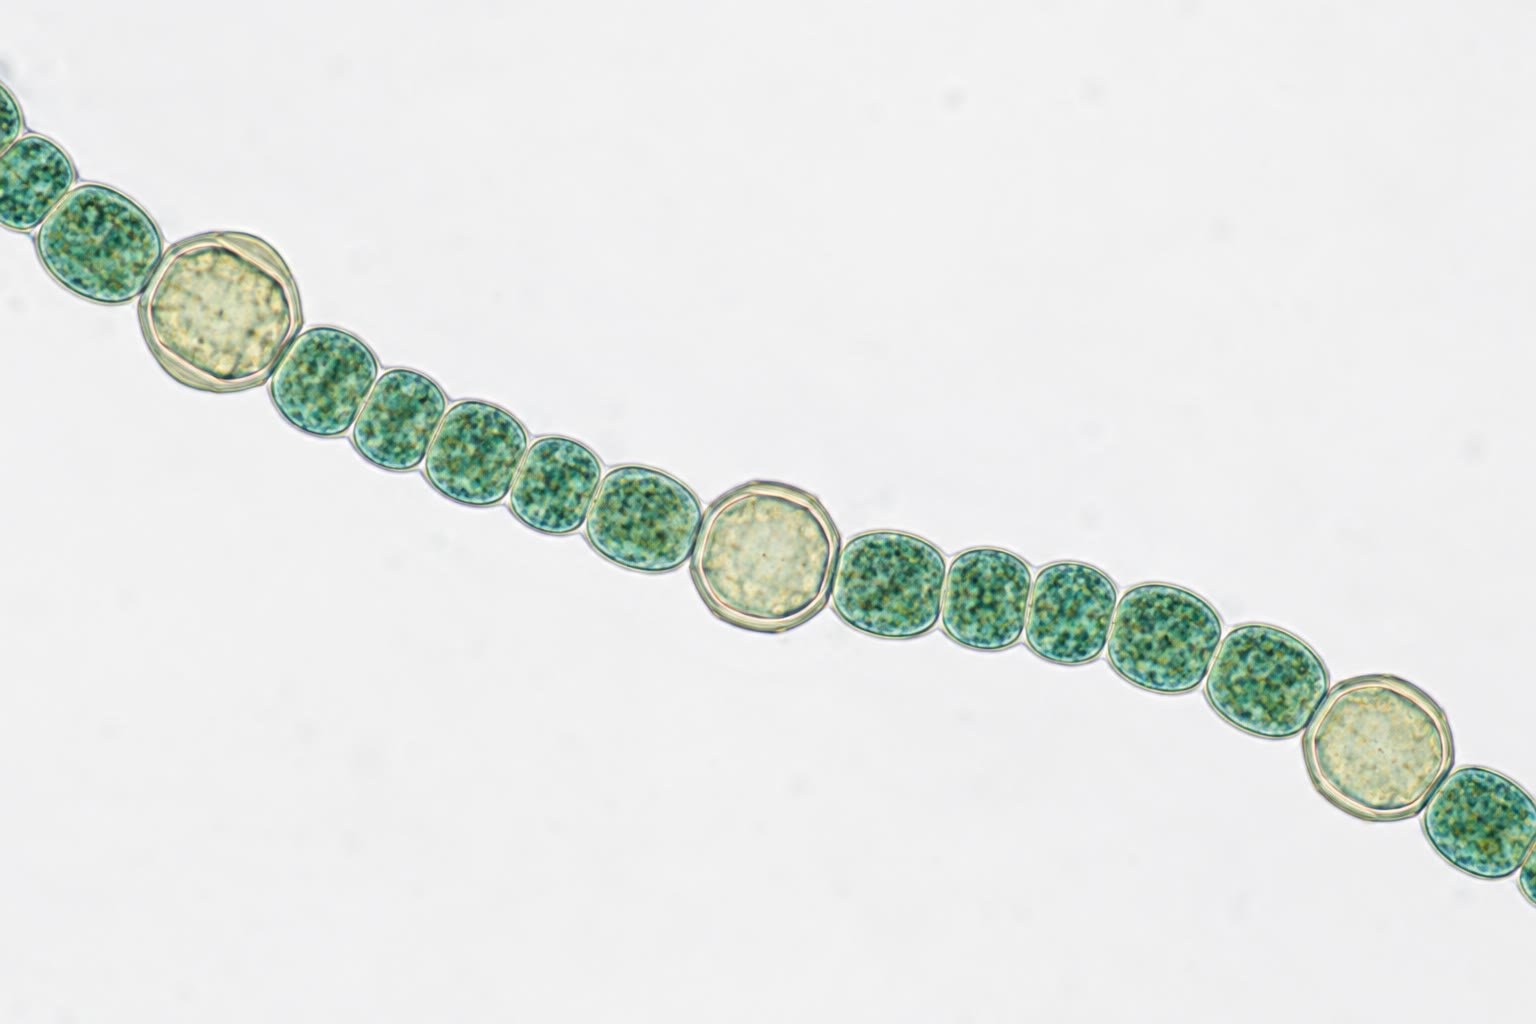
\includegraphics[width=0.62\linewidth]{images/book4/ai/b4-01-anabaena.jpg}

{\small Satu filamen \emph{Anabaena}: untaian sel hijau yang
berfotosintesis, disela heterosista yang lebih besar dan lebih pucat,
yaitu sel yang memfiksasi nitrogen.}
\end{omfigure}

\begin{remark}[Dormansi]\label{rem:b2:unicellular-diversity:spores}
Beberapa batang Gram positif (\emph{Bacillus}, \emph{Clostridium})
menjawab kelaparan dengan membangun sebuah \emph{endospora}: satu
salinan kromosomnya yang terbungkus beberapa mantel tanpa air, lengai
secara metabolik, tahan terhadap pendidihan, radiasi, dan kekeringan
berabad-abad, yang berkecambah ketika keadaannya pulih. Banyak \omterm{def:b2:unicellular-diversity:protist}{protista}
melakukan hal yang sama dengan sebuah \emph{sista}. Dormansi adalah
cara lain bertahan pada musim yang buruk, di samping kemampuan bergerak.
\end{remark}

\section{Organisme bersel tunggal yang eukariot}

\begin{definition}[Protista: sebuah tingkatan, bukan sebuah kelompok]\label{def:b2:unicellular-diversity:protist}
\emph{Protista}\index{protista} adalah eukariot yang bukan hewan, bukan
tumbuhan darat, dan bukan fungi --- kebanyakan \omterm{def:b2:unicellular-diversity:unicellular}{bersel tunggal}, sebagian
\omterm{def:b2:unicellular-diversity:unicellular}{berkoloni}, sedikit (ganggang cokelat raksasa) \omterm{def:b2:unicellular-diversity:unicellular}{bersel banyak}. Mereka
berbagi sel eukariot dari jilid Tahun ke-1 (nukleus,
mitokondria, endomembran, sitoskeleton, dan silia $9+2$) dan tidak
berbagi apa pun lagi yang khas: garis keturunan yang memuat mereka sama berjauhannya satu
sama lain seperti jarak hewan dari tumbuhan. Alga hijau segaris dengan
tumbuhan darat; diatom dan alga cokelat membentuk garis keturunan
sendiri; siliata, dinoflagelata, dan parasit malaria membentuk garis
yang lain; amuba dan jamur lendir lebih dekat kepada hewan dan fungi
daripada kepada semuanya itu. Sebutan itu menamai sebuah taraf
pengorganisasian --- sel eukariot yang hidup sendiri --- bukan sebuah
cabang pohonnya.
\end{definition}

\begin{example}[Empat cara menjadi sel eukariot yang hidup sendiri]\label{ex:b2:unicellular-diversity:four}
\emph{Chlamydomonas}: alga hijau bulat telur berdinding glikoprotein
tanpa selulosa, dengan satu kloroplas berbentuk cawan, sebuah bintik
mata jingga yang menaungi pengindera cahaya sehingga selnya mengetahui
dari arah mana cahayanya datang sembari berputar, dan dua flagelum di
ujung depan yang mengayuh seperti gaya dada; ia seorang fototrof.
\emph{Paramecium}: seekor siliata, seluruh permukaannya berdenyut oleh
silia dalam gelombang yang terpadu, sebuah alur mulut yang menyapu
bakteri ke dalam vakuola makanan, dua \omterm{prop:b2:unicellular-diversity:osmoregulation}{vakuola kontraktil}, dan dua macam
nukleus --- sebuah \emph{mikronukleus} kecil yang bersifat nutfah dan
sebuah \emph{makronukleus} besar yang bekerja dengan ratusan salinan
tiap gennya; ia seorang fagotrof. \emph{Amoeba}: tanpa dinding, tanpa
bentuk tetap, bergerak dan makan dengan \emph{pseudopodium} yang
didorong keluar oleh polimerisasi aktin. Diatom: sel berfotosintesis
yang terkurung dalam dua keping silika yang saling menindih bagaikan
kotak dan tutupnya, begitu berhias liang sehingga cangkangnya pernah
dipakai menguji lensa mikroskop; ketika membelah, tiap anaknya menyimpan
satu keping lalu membuat keping dalam yang baru dan lebih kecil.
\end{example}

\begin{omfigure}
\begin{tikzpicture}[every node/.style={font=\scriptsize}]
  % Paramecium outline (slipper)
  \draw[thick, fill=omProp!8] plot[smooth cycle, tension=0.8] coordinates {(0,0) (1.5,0.9) (3.5,1.1) (5.5,0.7) (6.4,0) (5.5,-0.8) (3.5,-1.1) (1.5,-0.9)};
  % cilia
  \foreach \t in {3,9,...,357} {
    \pgfmathsetmacro{\cx}{3.2+3.25*cos(\t)}
    \pgfmathsetmacro{\cy}{1.08*sin(\t)}
    \pgfmathsetmacro{\dx}{3.2+3.55*cos(\t)}
    \pgfmathsetmacro{\dy}{1.32*sin(\t)}
    \draw[gray] (\cx,\cy) -- (\dx,\dy);
  }
  % macronucleus and micronucleus
  \draw[thick, fill=omDef!40] (3.2,0.05) ellipse (0.9 and 0.45);
  \fill[omDef!90!black] (2.4,0.55) circle (0.13);
  % oral groove and gullet
  \draw[thick, omThm] (4.3,-0.95) .. controls (3.6,-0.5) and (3.3,-0.2) .. (3.0,-0.35);
  \fill[omThm!30] (2.9,-0.45) circle (0.16);
  % food vacuoles
  \foreach \p in {(1.4,-0.3),(1.0,0.35),(4.8,0.35)} \draw[thick, omExo!80!black, fill=omExo!30] \p circle (0.17);
  % contractile vacuoles
  \foreach \c in {(1.2,0.0),(5.2,-0.2)} {
    \draw[thick, omDef] \c circle (0.28);
    \foreach \a in {0,60,...,300} \draw[omDef] \c ++(\a:0.28) -- ++(\a:0.22);
  }
  % labels
  \draw (2.4,0.55) -- (2.7,1.6) node[above] {mikronukleus};
  \draw (3.6,0.3) -- (4.8,1.6) node[above] {makronukleus};
  \draw (1.2,0.28) -- (0.3,1.5) node[above, align=center] {vakuola kontraktil\\(berkanal jejari)};
  \draw (5.2,-0.48) -- (6.5,-1.5) node[below] {vakuola kontraktil};
  \draw (4.3,-0.95) -- (4.7,-1.75) node[below] {alur mulut};
  \draw (2.9,-0.61) -- (2.7,-1.6) node[below, align=center] {kerongkongan dan vakuola\\makanan yang sedang terbentuk};
  \draw (1.4,-0.47) -- (0.0,-1.5) node[below] {vakuola makanan};
  \draw (6.35,0.4) -- (6.9,1.2) node[above, align=center] {silia};
\end{tikzpicture}

{\small \emph{Paramecium}, skematik: korteks bersilia, kedua
nukleusnya, alur mulut yang menuju kerongkongan tempat vakuola makanan
terbentuk, dan kedua \omterm{prop:b2:unicellular-diversity:osmoregulation}{vakuola kontraktil} berbentuk bintang yang
mengeluarkan air yang didorong masuk oleh osmosis.}
\end{omfigure}

\begin{omfigure}
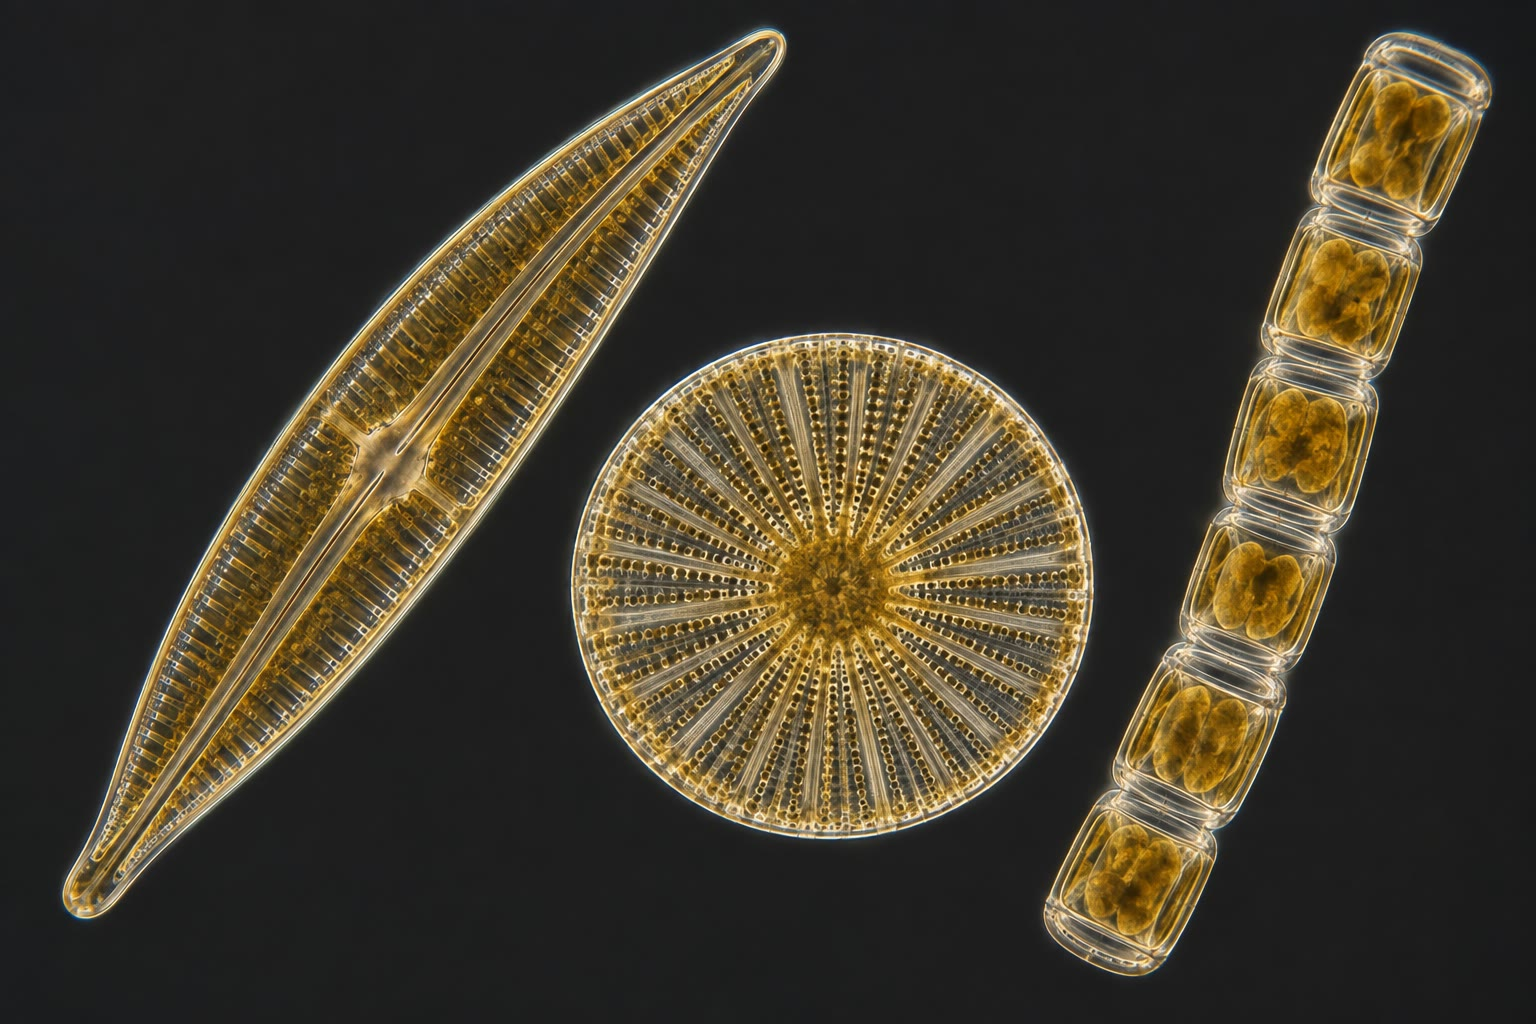
\includegraphics[width=0.6\linewidth]{images/book4/ai/b4-01-diatoms.jpg}

{\small Diatom dilihat dengan mikroskopi medan gelap: tiap selnya
tinggal di dalam cangkang silika berkeping dua, berpola liang yang
menjadi jalan pertukarannya dengan air.}
\end{omfigure}

\begin{definition}[Ragam cara makan]\label{def:b2:unicellular-diversity:nutrition}
\index{fagotrofi}\index{osmotrofi}\index{miksotrofi}
Sebuah eukariot \omterm{def:b2:unicellular-diversity:unicellular}{bersel tunggal} makan dengan salah satu dari tiga cara,
atau dengan dua cara sekaligus. \emph{Fototrofi}: ia memiliki kloroplas
dan membuat sendiri bahan organiknya dari cahaya dan $\mathrm{CO_2}$
(alga hijau, diatom, dinoflagelata). \emph{Fagotrofi}: ia menelan
butiran --- bakteri, \omterm{def:b2:unicellular-diversity:protist}{protista} lain --- ke dalam vakuola makanan tempat
enzim lisosom mencernanya (amuba, siliata, koanoflagelata).
\emph{Osmotrofi}: ia menyerap molekul terlarut menyeberangi membrannya,
kerap sesudah menyekresikan enzim ke luar (ragi, banyak parasit).
\emph{Miksotrof} seperti \emph{Euglena} berfotosintesis di dalam terang
dan makan di dalam gelap. \omterm{def:b2:unicellular-diversity:prokaryote}{Prokariot} tidak dapat berfagositosis:
dindingnya melarang, dan itulah sebabnya \omterm{def:b2:unicellular-diversity:prokaryote}{prokariot} tidak pernah menjadi
pemangsa lewat penelanan.
\end{definition}

\begin{proposition}[Pengaturan osmosis di air tawar]\label{prop:b2:unicellular-diversity:osmoregulation}
\index{vakuola kontraktil}
\omterm{def:b2:unicellular-diversity:protist}{Protista} air tawar jauh lebih asin di dalamnya (sekitar \qty{100}{mmol/L}
zat terlarut) daripada kolamnya (kira-kira \qty{1}{mmol/L}), dan
membrannya melewatkan air. Maka air terus-menerus masuk secara osmosis,
dengan laju sebanding dengan luas permukaannya dan dengan selisih
tekanan osmosisnya $\Delta\Pi = RT\,\Delta c$ --- kira-kira
\qty{2.4}{bar} untuk angka di atas. Sel berdinding menahannya dengan
turgor; sel telanjang akan menggembung lalu pecah dalam hitungan menit.
\emph{\omterm{prop:b2:unicellular-diversity:osmoregulation}{Vakuola kontraktil}} adalah jawabannya: sebuah waduk yang disuapi
kanal jejari, yang terisi air yang dipompa masuk oleh pengangkut
bertenaga proton lalu mengerut, mengeluarkan airnya lewat sebuah liang,
tiap beberapa sekon sampai tiap beberapa menit. Seekor
\emph{Paramecium} melewatkan air sebanyak volumenya sendiri tiap
setengah jam; kerabatnya di laut, di dalam medium yang seasin dirinya,
sama sekali tidak memiliki \omterm{prop:b2:unicellular-diversity:osmoregulation}{vakuola kontraktil}.
\end{proposition}

\section{Fisika seorang perenang kecil}

\begin{proposition}[Kehidupan pada bilangan Reynolds kecil]\label{prop:b2:unicellular-diversity:reynolds}
\index{bilangan Reynolds}
\emph{\omterm{prop:b2:unicellular-diversity:reynolds}{Bilangan Reynolds}} $Re = \rho v L/\eta$ membandingkan gaya
kelembaman dengan gaya kental bagi benda berukuran $L$ yang bergerak
pada kelajuan $v$ di dalam fluida bermassa jenis $\rho$ dan
berkekentalan $\eta$. Bagi perenang manusia nilainya sekitar $10^6$;
bagi \emph{Paramecium} (\qty{200}{\micro m}, \qty{1}{mm/s}) nilainya
0,2, dan bagi sebuah bakteri $10^{-5}$. Di bawah $Re \approx 1$
kelembaman tidak berperan: sel yang berhenti berdenyut berhenti
bergerak dalam jarak satu nanometer, air terasa seperti sirup kental,
dan gerak bolak-balik (kayuhan yang sama maju dan mundur) tidak
menghasilkan perpindahan neto. Maka perenang kecil memakai kayuhan yang
tidak bolak-balik: heliks berputar flagelum bakteri, denyut tak setangkup
sebuah silia (kayuhan tenaga yang kaku, kayuhan pulih yang melengkung),
gaya dada \emph{Chlamydomonas}.
\end{proposition}

\begin{theorem}[Hukum Stokes dan pengendapan]\label{thm:b2:unicellular-diversity:stokes}
\index{hukum Stokes}
Sebuah bola berjari-jari $r$ dan bermassa jenis $\rho_{\text{sel}}$
yang bergerak perlahan menembus fluida berkekentalan $\eta$ merasakan
seretan $F = 6\pi\eta r v$. Dibiarkan sendiri di dalam air bermassa
jenis $\rho$, ia tenggelam pada kelajuan terminal
\[
v_s = \frac{2\,r^2\,(\rho_{\text{sel}} - \rho)\,g}{9\eta},
\]
yang sebanding dengan kuadrat jari-jarinya: sel sepuluh kali lebih
besar tenggelam seratus kali lebih cepat. Inilah sebabnya fitoplankton
berukuran kecil, sebabnya diatom mengusung duri dan tetes minyak, dan
sebabnya \emph{Chlamydomonas} yang berhenti berenang tenggelam ke luar
dari cahaya dalam beberapa hari.
\end{theorem}
\begin{proof}
Pada kelajuan terminal, seretannya mengimbangi berat semunya (berat
dikurangi gaya apung): $6\pi\eta r v_s = \tfrac{4}{3}\pi r^3
(\rho_{\text{sel}} - \rho) g$. Memecahkannya untuk $v_s$ memberikan
rumusnya. Hukum seretannya sendiri diturunkan dalam seri fisika untuk
$Re \ll 1$; di sini ia diterima sebagaimana adanya.
\end{proof}

\begin{example}[Jatuhnya sebuah diatom]\label{ex:b2:unicellular-diversity:fall}
Sebuah diatom sentrik berjari-jari \qty{10}{\micro m}, \qty{100}{kg/m^3}
lebih padat daripada air laut ($\eta = \qty{1e-3}{Pa.s}$), tenggelam pada
$v_s = 2\times 10^{-10}\times 100\times 9.81/(9\times 10^{-3}) =
\qty{2.2e-5}{m/s}$, kira-kira \qty{2}{m} tiap hari: ia akan meninggalkan
lapisan bercahaya setebal \qty{50}{m} dalam waktu kurang dari sebulan.
Populasinya bertahan karena olakan mengaduk airnya, karena tetes minyak
dan massa jenis yang rendah memangkas $\rho_{\text{sel}} - \rho$, dan
karena sel yang tenggelam lalu membelah di tengah jalan meninggalkan
keturunan yang terangkat kembali.
\end{example}

\begin{omfigure}
\begin{tikzpicture}
\begin{axis}[
  width=0.8\linewidth, height=6.0cm,
  axis x line=bottom, axis y line=left,
  xmode=log, ymode=log,
  xmin=0.5, xmax=200, ymin=1e-3, ymax=1e4,
  xlabel={jari-jari (\unit{\micro m})}, ylabel={kelajuan pengendapan (\unit{\micro m/s})},
  xlabel style={font=\small, at={(axis description cs:0.5,-0.1)}, anchor=north},
  ylabel style={font=\small},
  tick label style={font=\small},
  clip=false,
]
\addplot[very thick, omDef, domain=0.5:200, samples=40] {0.218*x^2};
\addplot[only marks, mark=*, mark size=1.8pt, omThm] coordinates {(1,0.218) (10,21.8) (100,2180)};
\node[font=\scriptsize, anchor=west] at (axis cs:1.15,0.218) {bakteri};
\node[font=\scriptsize, anchor=west] at (axis cs:11.5,21.8) {diatom};
\node[font=\scriptsize, anchor=east] at (axis cs:85,2180) {protista besar};
\end{axis}
\end{tikzpicture}

{\small Kelajuan pengendapan Stokes terhadap jari-jari bagi sel yang
\qty{100}{kg/m^3} lebih padat daripada air. Kemiringan 2 pada sumbu
logaritmik adalah hukum $r^2$: bakteri tenggelam satu sentimeter tiap
hari, \omterm{def:b2:unicellular-diversity:protist}{protista} besar beberapa meter tiap jam.}
\end{omfigure}

\section{Perkembangbiakan dan seks di dalam satu sel}

\begin{definition}[Ragam pembelahan]\label{def:b2:unicellular-diversity:division}
\index{pembelahan biner}\index{pertunasan}\index{pembelahan ganda}
\omterm{def:b2:unicellular-diversity:unicellular}{Organisme bersel tunggal} berbiak dengan membelah. \emph{Pembelahan
biner}: selnya tumbuh sampai dua kali ukurannya lalu terbelah menjadi
dua sel anak yang sama besar (bakteri, \emph{Paramecium},
\emph{Amoeba}). \emph{Pertunasan}: seorang anak kecil tumbuh keluar
dari induknya lalu melepaskan diri (ragi; induknya menyimpan sebuah
parut dan dapat bertunas sekitar dua puluh kali). \emph{Pembelahan
ganda}: selnya tumbuh besar, lalu membelah beberapa kali berturut-turut
dengan cepat di dalam dinding induknya dan melepaskan 4, 8, 16, atau
lebih anak sekaligus (\emph{Chlamydomonas}, parasit malaria di dalam
sel darah merah). Pada keadaan tetap, cacah selnya tumbuh secara
eksponensial, $N(t) = N_0\,2^{t/T}$ dengan $T$ sebagai \emph{waktu
generasi}\index{waktu generasi}: dua puluh menit bagi \emph{E.~coli}
dalam medium kaya, sehari bagi banyak alga, sepekan bagi sebagian
siliata. (Pertumbuhan sebagai fungsi makanan dibahas dalam
\cref{ch:b2:microbial-metabolism}.)
\end{definition}

\begin{proposition}[Seks tanpa perkembangbiakan: konjugasi pada \emph{Paramecium}]\label{prop:b2:unicellular-diversity:conjugation}
\index{konjugasi!siliata}
Dua \emph{Paramecium} bertipe kawin saling melengkapi bergabung lewat
permukaan mulutnya. Pada masing-masing, mikronukleus diploidnya
menjalani meiosis menjadi empat nukleus haploid, tiga di antaranya
merosot; yang bertahan membelah secara mitosis menjadi satu nukleus
tetap dan satu nukleus pindah, lalu kedua selnya bertukar nukleus
pindah menyeberangi sambungannya. Tiap selnya kemudian meleburkan
nukleus tetapnya dengan nukleus yang diterimanya, dan kedua pasangannya
berpisah, masing-masing dengan mikronukleus diploid baru yang segenotipe
dengan pasangannya. Makronukleus lamanya terurai dan sebuah makronukleus
baru dibangun dari mikronukleus barunya. Tidak ada sel baru yang dibuat:
konjugasi adalah pencampuran genetik --- meiosis dan pembuahan,
\cref{ch:b2:meiosis-heredity} --- yang terlepas dari pelipatgandaan.
Konjugasi bakteri, yang memindahkan sebuah \omterm{def:b2:unicellular-diversity:prokaryote}{plasmid} satu arah dari
pemberi ke penerima, adalah proses lain dengan nama yang sama
(\cref{ch:b2:genome-diversification}).
\end{proposition}

\begin{omfigure}
\begin{tikzpicture}[every node/.style={font=\scriptsize}]
  \foreach \i/\x in {0/0,1/3.6,2/7.2,3/10.8} {
    \draw[thick, fill=omProp!8] (\x,0.55) ellipse (1.0 and 0.5);
    \draw[thick, fill=omProp!8] (\x,-0.55) ellipse (1.0 and 0.5);
  }
  % stage 0: two cells, diploid micronuclei 2n
  \fill[omDef!90!black] (0,0.55) circle (0.12); \node[right] at (0.15,0.55) {$2n$};
  \fill[omDef!90!black] (0,-0.55) circle (0.12); \node[right] at (0.15,-0.55) {$2n$};
  \node[below, align=center] at (0,-1.15) {dua sel bergabung};
  % stage 1: meiosis, 4 haploid, 3 degenerate
  \foreach \dy in {0.55,-0.55} {
    \fill[omDef!90!black] (3.6-0.3,\dy+0.15) circle (0.08);
    \fill[gray!60] (3.6+0.1,\dy+0.2) circle (0.06);
    \fill[gray!60] (3.6+0.3,\dy-0.05) circle (0.06);
    \fill[gray!60] (3.6-0.1,\dy-0.25) circle (0.06);
  }
  \node[below, align=center] at (3.6,-1.15) {meiosis:\\4 nukleus haploid,\\tiga merosot};
  % stage 2: mitosis, exchange
  \foreach \dy in {0.55,-0.55} {
    \fill[omDef!90!black] (7.2-0.35,\dy) circle (0.08);
    \fill[omThm] (7.2+0.35,\dy) circle (0.08);
  }
  \draw[->, thick, omThm] (7.55,0.45) -- (7.55,-0.45);
  \draw[->, thick, omThm] (6.85,-0.45) -- (6.85,0.45);
  \node[below, align=center] at (7.2,-1.15) {mitosis; nukleus\\pindah (merah)\\dipertukarkan};
  % stage 3: fusion 2n
  \fill[omDef!90!black] (10.8,0.55) circle (0.12); \node[right] at (10.95,0.55) {$2n$};
  \fill[omDef!90!black] (10.8,-0.55) circle (0.12); \node[right] at (10.95,-0.55) {$2n$};
  \node[below, align=center] at (10.8,-1.15) {pembuahan:\\nukleus diploid baru\\yang serupa; selnya berpisah};
  \foreach \x in {1.3,4.9,8.5} \draw[->, thick, gray] (\x,0) -- (\x+1.0,0);
\end{tikzpicture}

{\small Konjugasi pada \emph{Paramecium}. Dua sel bertukar nukleus
haploid lalu berpisah, masing-masing mengusung mikronukleus diploid
hasil rekombinasi; cacah selnya tidak berubah.}
\end{omfigure}

\section{Menuju kehidupan bersel banyak}

\begin{proposition}[Deret volvosin]\label{prop:b2:unicellular-diversity:volvox}
\index{Volvox@\emph{Volvox}}\index{bersel banyak, asal-usul}
Di antara alga hijau ada satu garis keturunan yang memperagakan, pada
spesies yang masih hidup, tahap-tahap dari satu sel menuju satu tubuh.
\emph{Chlamydomonas} hidup sendiri. \emph{Gonium} adalah lempeng datar
berisi 4 sampai 16 sel serupa yang berenang bersama. \emph{Pandorina}
dan \emph{Eudorina} adalah bola berongga berisi 16 sampai 32 sel, masih
semuanya serupa, masing-masing sanggup mendirikan koloni baru.
\emph{Pleodorina} memiliki beberapa sel kecil yang hanya berenang dan
tidak pernah membelah. \emph{Volvox} adalah bola berisi \num{500}
sampai \num{50000} sel soma kecil berflagelum, yang akan mati bersama
koloninya, mengelilingi segelintir sel nutfah besar (gonidium) yang
membelah membentuk bola anak di dalam induknya. Sel soma dan sel nutfah
telah muncul: inilah ambang kehidupan \omterm{def:b2:unicellular-diversity:unicellular}{bersel banyak}, yang dilintasi
garis keturunan ini sekitar \num{200} juta tahun silam dan, secara
bebas, sedikitnya dua puluh lima kali di tempat lain pada pohon
kehidupan --- pada hewan, tumbuhan, fungi, alga cokelat, alga merah,
dan beberapa kelompok bakteri.
\end{proposition}
\begin{proof}[Bukti eksperimental]
Filogeni molekuler alga volvosin, yang dibangun dari puluhan gen,
menempatkan \emph{Chlamydomonas} di pangkalnya dan \emph{Volvox} di
ujungnya, dengan bentuk \omterm{def:b2:unicellular-diversity:unicellular}{berkoloni} di antaranya dan cacah selnya
meningkat sepanjang cabangnya; genom \emph{Volvox carteri} (2010)
berbeda dari genom \emph{Chlamydomonas} hanya dalam beberapa ratus gen,
terutama gen matriks ekstrasel yang menahan sel-selnya dan gen pengatur
yang membungkam pembelahan pada sel soma. Peralihan itu menuntut bahan
genetik baru yang luar biasa sedikit.
\end{proof}

\begin{omfigure}
\begin{tikzpicture}[every node/.style={font=\scriptsize}]
  % Chlamydomonas
  \draw[thick, fill=omProp!25] (0,0) circle (0.22);
  \node[below=0.35cm, align=center] at (0,0) {\emph{Chlamydomonas}\\1 sel};
  % Gonium plate
  \begin{scope}[xshift=2.2cm]
    \foreach \x in {-0.3,0,0.3} \foreach \y in {-0.3,0,0.3} \draw[thick, fill=omProp!25] (\x,\y) circle (0.14);
    \draw[gray, dashed] (-0.55,-0.55) rectangle (0.55,0.55);
    \node[below=0.7cm, align=center] at (0,0) {\emph{Gonium}\\lempeng 8--16};
  \end{scope}
  % Eudorina ball
  \begin{scope}[xshift=4.5cm]
    \draw[gray, dashed] (0,0) circle (0.6);
    \foreach \a in {0,45,...,315} \draw[thick, fill=omProp!25] (\a:0.55) circle (0.13);
    \draw[thick, fill=omProp!25] (0,0.1) circle (0.13);
    \node[below=0.7cm, align=center] at (0,0) {\emph{Eudorina}\\bola berisi 32,\\semuanya serupa};
  \end{scope}
  % Pleodorina
  \begin{scope}[xshift=7.4cm]
    \draw[gray, dashed] (0,0) circle (0.7);
    \foreach \a in {0,30,...,330} \draw[thick, fill=omProp!25] (\a:0.62) circle (0.09);
    \foreach \a in {60,180,300} \draw[thick, fill=omProp!60] (\a:0.62) circle (0.14);
    \node[below=0.8cm, align=center] at (0,0) {\emph{Pleodorina}\\beberapa sel\\hanya berenang};
  \end{scope}
  % Volvox
  \begin{scope}[xshift=10.6cm]
    \draw[thick, fill=omProp!6] (0,0) circle (0.95);
    \foreach \a in {0,12,...,348} \fill[omProp!70] (\a:0.9) circle (0.035);
    \foreach \a in {0,12,...,348} \fill[omProp!50] (\a:0.72) circle (0.03);
    \foreach \p in {(0.25,0.2),(-0.3,-0.25),(0.1,-0.4),(-0.2,0.35)} \draw[thick, omThm, fill=omThm!40] \p circle (0.13);
    \node[below=1.05cm, align=center] at (0,0) {\emph{Volvox}\\ribuan sel soma\\dan beberapa sel nutfah (merah)};
  \end{scope}
  \foreach \x in {0.5,3.0,5.3,8.3} \draw[->, gray] (\x,0) -- (\x+0.6,0);
\end{tikzpicture}

{\small Deret volvosin: satu sel, satu lempeng, satu bola berongga
berisi sel serupa, satu bola yang sebagian selnya telah melepaskan
pembelahan, dan \emph{Volvox}, tempat ribuan sel soma yang fana
mengelilingi beberapa sel nutfah.}
\end{omfigure}

\begin{omfigure}
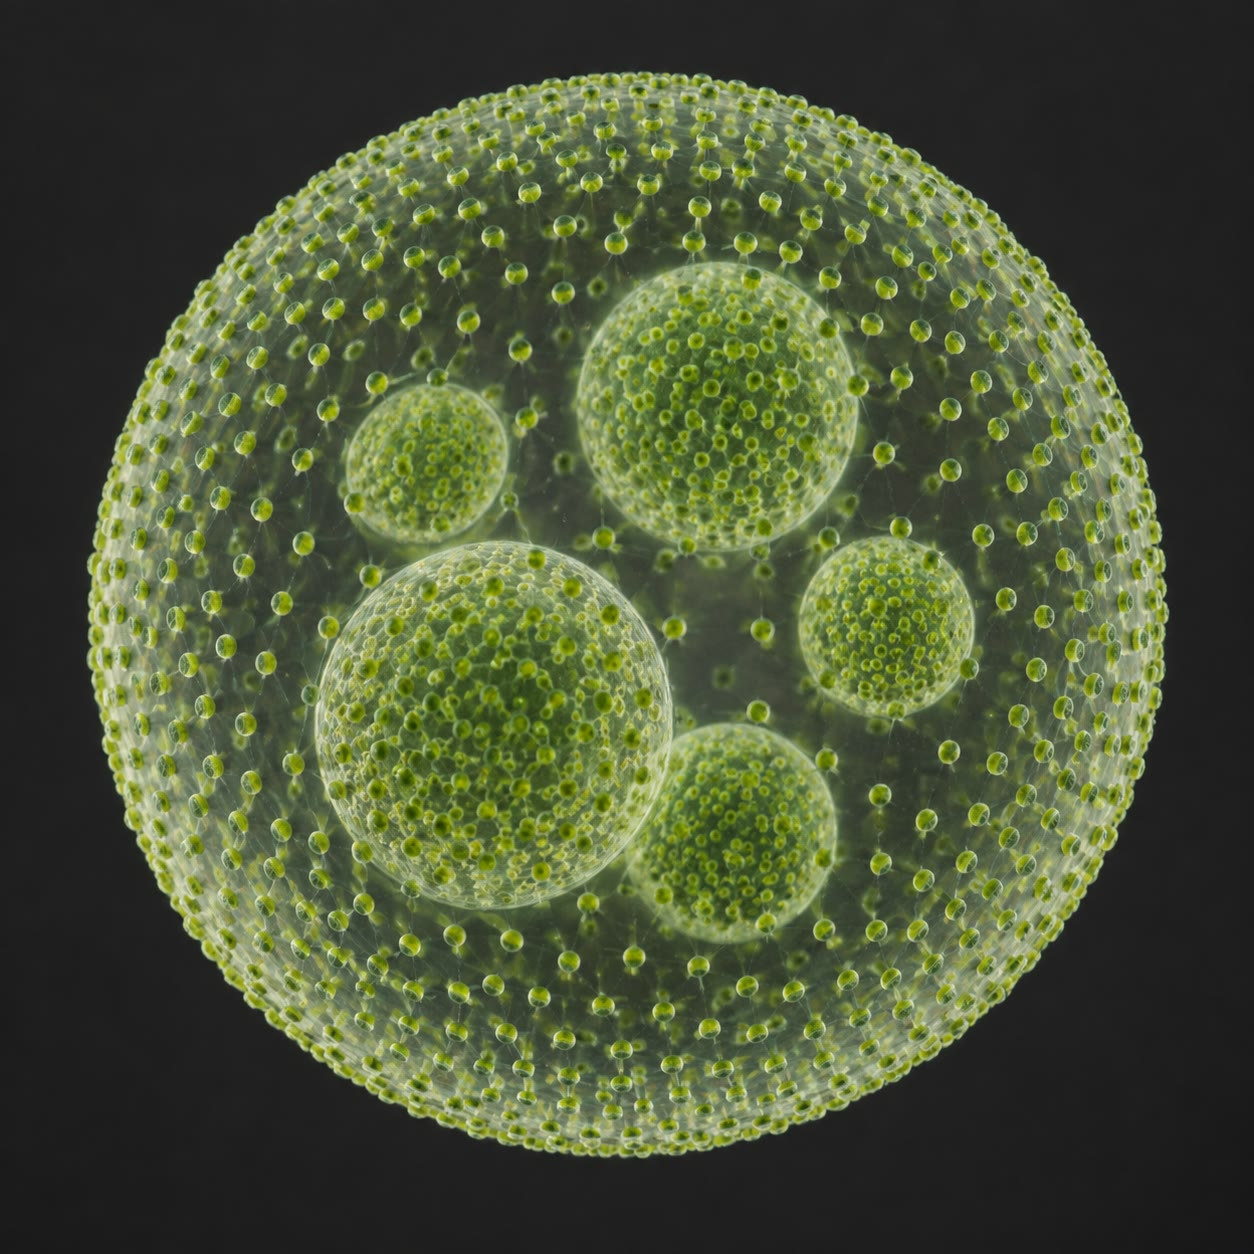
\includegraphics[width=0.55\linewidth]{images/book4/ai/b4-01-volvox.jpg}

{\small Sebuah koloni \emph{Volvox}: bola hijau berongga berisi sel
berflagelum, dengan koloni anak yang tumbuh di dalamnya.}
\end{omfigure}

\begin{remark}[Mengapa membagi kerja?]\label{rem:b2:unicellular-diversity:whydivide}
Pada alga ini sebuah sel tidak dapat berenang dan membelah sekaligus:
badan basal yang menambatkan flagelumnya dibutuhkan untuk menata
gelendongnya. Sel tunggal berganti-ganti; koloni kecil sanggup berhenti
berenang selama semua selnya membelah; koloni besar akan tenggelam ke
luar dari cahaya (\omterm{thm:b2:unicellular-diversity:stokes}{hukum Stokes}, \cref{thm:b2:unicellular-diversity:stokes})
selama berjam-jam pembelahannya. Melewati ukuran tertentu, menjaga
sebagian sel tetap berenang sementara yang lain membelah sepadan dengan
hilangnya keturunan mereka --- dan lahirlah soma. Koanoflagelata,
flagelata berkerah yang selnya adalah salinan sel pemakan spons,
memperlihatkan langkah pertama yang sama pada cabang yang menuju hewan.
\end{remark}

\section{Latihan}

\begin{exercise}[$\star$]\label{exo:b2:unicellular-diversity:1}
Definisikan \omterm{def:b2:unicellular-diversity:unicellular}{bersel tunggal}, \omterm{def:b2:unicellular-diversity:unicellular}{berkoloni}, dan \omterm{def:b2:unicellular-diversity:unicellular}{bersel banyak}, lalu
tempatkan \emph{E.~coli}, \emph{Gonium}, \emph{Volvox}, dan sebuah sel
ragi pada golongan yang tepat beserta alasannya.
\end{exercise}

\begin{exercise}[$\star$]\label{exo:b2:unicellular-diversity:2}
Hitunglah \omterm{prop:b2:unicellular-diversity:surface}{rasio permukaan terhadap volume} sebuah kokus berjari-jari
\qty{0.5}{\micro m} dan sebuah \omterm{def:b2:unicellular-diversity:protist}{protista} bola berjari-jari
\qty{50}{\micro m}. Mana yang bernapas lebih cepat tiap satuan
sitoplasma, dan mengapa?
\end{exercise}

\begin{exercise}[$\star$]\label{exo:b2:unicellular-diversity:3}
Sebutkan tiga perbedaan struktural antara sebuah bakteri dan sebuah
eukariot \omterm{def:b2:unicellular-diversity:unicellular}{bersel tunggal}, serta satu hal yang tidak dapat dikerjakan
bakteri tetapi dapat dikerjakan amuba.
\end{exercise}

\begin{exercise}[$\star$]\label{exo:b2:unicellular-diversity:4}
Sebutkan fungsi tiap struktur \emph{Paramecium} berikut: silia, alur
mulut, vakuola makanan, \omterm{prop:b2:unicellular-diversity:osmoregulation}{vakuola kontraktil}, makronukleus,
mikronukleus.
\end{exercise}

\begin{exercise}[$\star\star$]\label{exo:b2:unicellular-diversity:5}
Dengan $D = \qty{5e-10}{m^2/s}$ bagi sebuah metabolit di dalam
sitoplasma, berapa lama difusi menyeberangi bakteri \qty{1}{\micro m}
dan menyeberangi amuba \qty{500}{\micro m}? Berilah ulasan tentang apa
yang harus dikerjakan amubanya tetapi tidak perlu dikerjakan bakterinya.
\end{exercise}

\begin{exercise}[$\star\star$]\label{exo:b2:unicellular-diversity:6}
Hitunglah \omterm{prop:b2:unicellular-diversity:reynolds}{bilangan Reynolds} sebuah \emph{Paramecium} (\qty{200}{\micro
m}, \qty{1}{mm/s}), sebuah bakteri (\qty{2}{\micro m}, \qty{20}{\micro
m/s}), dan seorang perenang manusia (\qty{2}{m}, \qty{1}{m/s}), dengan
$\rho = \qty{1000}{kg/m^3}$ dan $\eta = \qty{1e-3}{Pa.s}$. Mengapa
perenangnya dapat meluncur sesudah satu kayuhan sedangkan bakterinya tidak?
\end{exercise}

\begin{exercise}[$\star\star$]\label{exo:b2:unicellular-diversity:7}
Sebuah diatom berjari-jari \qty{10}{\micro m} adalah \qty{100}{kg/m^3}
lebih padat daripada air. Hitunglah kelajuan pengendapannya dan waktu
untuk jatuh sejauh \qty{50}{m}. Dengan faktor berapa waktunya berubah
jika selnya memerohkan jari-jarinya? Jika ia memangkas kelebihan massa
jenisnya menjadi \qty{20}{kg/m^3}?
\end{exercise}

\begin{exercise}[$\star\star$]\label{exo:b2:unicellular-diversity:8}
Modelkan sebuah \emph{Paramecium} sebagai elipsoid dengan setengah
sumbu \num{100}, \num{25}, dan \qty{25}{\micro m} ($V = \tfrac{4}{3}\pi abc$).
Ia mengeluarkan air sebanyak volumenya sendiri tiap \qty{30}{min}.
Hitunglah aliran air yang masuk dalam \unit{\micro m^3/s} dan dalam
liter tiap sekon.
\end{exercise}

\begin{exercise}[$\star\star$]\label{exo:b2:unicellular-diversity:9}
Sebuah zat penarik berlipat dua kepekatannya sepanjang \qty{1}{mm}.
Berapakah selisih nisbi antara kedua ujung sebuah bakteri
\qty{1}{\micro m}? Antara awal dan akhir sebuah lari \qty{1}{s} pada
\qty{20}{\micro m/s}? Mencacah $N$ molekul memiliki galat nisbi
kira-kira $1/\sqrt{N}$: jelaskan mengapa bakterinya membandingkan waktu
dan bukan kedua sisinya.
\end{exercise}

\begin{exercise}[$\star\star\star$]\label{exo:b2:unicellular-diversity:10}
\emph{Thiomargarita namibiensis} adalah bakteri belerang berbentuk bola
bergaris tengah \qty{500}{\micro m} yang sitoplasmanya berupa selaput
setebal \qty{2}{\micro m} mengelilingi sebuah vakuola nitrat. Hitunglah
rasio permukaannya terhadap volume \emph{sitoplasma}nya lalu
bandingkan dengan \emph{E.~coli} (sebuah silinder berjari-jari
\qty{0.5}{\micro m}; abaikan kedua ujungnya). Jelaskan bagaimana
vakuolanya memungkinkannya sebesar itu, dan untuk apa nitratnya.
\end{exercise}

\begin{exercise}[$\star\star\star$]\label{exo:b2:unicellular-diversity:11}
Pada \emph{Volvox} sel somanya tidak pernah membelah dan mati bersama
koloninya. Dengan memakai kendala flagelasi dan \omterm{thm:b2:unicellular-diversity:stokes}{hukum Stokes}, jelaskan
mengapa sel semacam itu sepadan dimiliki koloni berisi \num{10000} sel
tetapi tidak pada koloni berisi 16 sel, dan mengapa sel nutfahnya
adalah sel terbesar pada bolanya.
\end{exercise}

\begin{exercise}[$\star\star\star$]\label{exo:b2:unicellular-diversity:12}
``\omterm{def:b2:unicellular-diversity:protist}{Protista} adalah sebuah tingkatan, bukan sebuah klad.'' Jelaskan
perbedaannya dengan garis keturunan yang disebut dalam bab ini, dan
katakan mengapa pernyataan yang sama benar bagi ``\omterm{def:b2:unicellular-diversity:prokaryote}{prokariot}'' dan salah
bagi ``sianobakteri''.
\end{exercise}

\section{Soal: Setetes Air Kolam}

\begin{problem}[{Soal akhir pekan --- sebuah contoh air kolam dicacah,
ditumbuhkan, dan dianalisis dari segi fisika yang mengatur selnya,
berakhir pada neraca air dan energi sebuah alga hijau}]
\label{pb:b2:unicellular-diversity:1}
Sebuah kolam \qty{1000}{m^3} diambil contohnya pada musim semi. Di bawah
mikroskop, sebuah bilik pencacah yang kisinya meliputi
\qty{1}{mm}$\times$\qty{1}{mm}
di bawah kaca penutup yang ditahan \qty{0.1}{mm} di atasnya memperlihatkan
24 sel \emph{Chlamydomonas} (bola berjari-jari \qty{5}{\micro m},
massa jenis \qty{1050}{kg/m^3}). Ambillah $\rho = \qty{1000}{kg/m^3}$,
$\eta = \qty{1e-3}{Pa.s}$, $g = \qty{9.81}{m/s^2}$, $R =
\qty{8.314}{J/mol/K}$, $T = \qty{293}{K}$, $D = \qty{1.9e-9}{m^2/s}$
bagi $\mathrm{CO_2}$ di dalam air.

\medskip
\noindent\textbf{Bagian I --- Pencacahan.}
\begin{enumerate}
  \item Hitunglah volume air di bawah kisinya, dalam mikroliter.
  \item Simpulkan kerapatan \emph{Chlamydomonas} di dalam kolamnya,
        dalam sel tiap mililiter.
  \item Hitunglah volume dan \omterm{prop:b2:unicellular-diversity:surface}{rasio permukaan terhadap volume} satu
        selnya.
  \item Berapa bagian volume air kolamnya yang ditempati sel-sel ini?
  \item Berapa banyak \emph{Chlamydomonas} yang dikandung kolamnya?
  \item Sebuah sianobakteri berfilamen juga hadir. Berikan dua ciri
        yang terlihat di bawah mikroskop yang membedakannya dari
        alganya.
\end{enumerate}

\medskip
\noindent\textbf{Bagian II --- Pertumbuhan.}
Contohnya disimpan dalam terang lalu dicacah lagi sesudah \qty{48}{h}:
\num{384} sel di bawah kisinya.
\begin{enumerate}[resume]
  \item Hitunglah \omterm{def:b2:unicellular-diversity:division}{waktu generasi} $T$.
  \item Hitunglah tetapan laju pertumbuhan $k$ dalam $N = N_0 e^{kt}$,
        dalam \unit{h^{-1}}.
  \item Berapa lama populasi kolamnya mencapai \qty{1e8}{} sel tiap
        mililiter pada laju ini?
  \item Berikan tiga alasan mengapa hal itu tidak akan terjadi.
  \item Jika selnya hanya tumbuh selama \qty{12}{h} siang hari dan sama
        sekali tidak tumbuh pada malam hari, berapa lama kenaikan yang
        sama itu berlangsung?
  \item \emph{Chlamydomonas} membelah secara \omterm{def:b2:unicellular-diversity:division}{pembelahan ganda}, melepaskan
        4, 8, atau 16 anak sekaligus. Jelaskan mengapa \omterm{def:b2:unicellular-diversity:division}{waktu generasi}
        tetap terdefinisi dengan baik oleh cacahnya.
\end{enumerate}

\medskip
\noindent\textbf{Bagian III --- Fisika selnya.}
\begin{enumerate}[resume]
  \item Hitunglah \omterm{prop:b2:unicellular-diversity:reynolds}{bilangan Reynolds} sebuah sel yang berenang pada
        \qty{100}{\micro m/s}.
  \item Sebuah sel bermassa $m$ yang berhenti mendenyutkan flagelumnya
        meluncur sejauh $mv/(6\pi\eta r)$. Hitunglah jarak itu.
  \item Hitunglah kelajuan pengendapan sebuah sel yang berhenti
        berenang.
  \item Bandingkan waktu untuk tenggelam \qty{1}{m} dengan waktu untuk
        berenang naik \qty{1}{m}.
  \item Kolamnya memuat \qty{10}{\micro mol/L} $\mathrm{CO_2}$
        terlarut. Hitunglah pasokan difusif maksimal
        $\mathrm{CO_2}$ ke sebuah sel, dalam molekul tiap sekon.
  \item Sebuah sel mengandung \qty{100}{pg} karbon dan melipatduakannya
        dalam satu generasi. Hitunglah purata permintaan karbonnya dalam
        molekul tiap sekon, dan rasio pasokan terhadap permintaannya.
  \item Ulangi perbandingannya bagi sel hipotetis berjari-jari
        \qty{50}{\micro m} dengan kerapatan karbon yang sama. Simpulkan.
\end{enumerate}

\medskip
\noindent\textbf{Bagian IV --- Air dan energi.}
Sitoplasmanya memuat \qty{100}{mmol/L} zat terlarut, kolamnya
\qty{1}{mmol/L}. Keterhantaran hidraulik membrannya adalah $L_p =
\qty{1e-14}{m.s^{-1}.Pa^{-1}}$ (fluks volume air tiap satuan luas tiap
satuan selisih tekanan). Menghidrolisis satu ATP menghasilkan
\qty{50}{kJ/mol}; memfiksasi satu atom karbon memakan tiga ATP.
\begin{enumerate}[resume]
  \item Hitunglah selisih tekanan osmosis menyeberangi membrannya.
  \item Hitunglah volume air yang masuk ke dalam selnya tiap sekon,
        dalam \unit{\micro m^3/s}.
  \item Tanpa \omterm{prop:b2:unicellular-diversity:osmoregulation}{vakuola kontraktil}, berapa lama selnya melipatduakan
        volumenya?
  \item Hitunglah daya minimal yang dibutuhkan untuk mengeluarkan air
        ini melawan tekanan osmosisnya.
  \item Ubahlah menjadi molekul ATP tiap sekon lalu bandingkan dengan
        ATP yang dibelanjakan selnya untuk fiksasi karbon (pertanyaan 18).
  \item Nyatakan hasilnya: aliran air yang masuk ke dalam selnya, waktu
        yang dibutuhkannya untuk pecah, dan bagian energinya yang
        dihabiskan untuk tetap kering.
\end{enumerate}
\end{problem}
